\documentclass[12pt,a4paper]{article}

\usepackage[utf8]{inputenc}
\usepackage{graphicx}
\usepackage{geometry}
\usepackage{amsmath}
\usepackage{amssymb}
\usepackage{hyperref}
\usepackage{float}
\usepackage{booktabs}
\usepackage{siunitx}
\usepackage{array}
\usepackage{caption}
\usepackage{subcaption}
\usepackage{color}

\geometry{
    a4paper,
    top=2.5cm,
    bottom=2.5cm,
    left=2.2cm,
    right=2.2cm
}

\hypersetup{
    colorlinks=true,
    linkcolor=blue,
    citecolor=blue,
    urlcolor=blue
}

\title{\textbf{Experiment 3: X-Ray Diffraction (XRD)}}

\author{\textbf{Yamulapalli Nandu Navadeep} \\
Roll No: IMS24267 \\
Advanced Physics Laboratory II (PHY-325)}

\date{Date of Experiment: 28 September 2026 \\
Date of Submission: \today}

\begin{document}

\maketitle

\section{Name of the Experiment}
X-Ray Diffraction (XRD): Determination of Lattice Parameters for Single Crystals and Powders by Analyzing XRD Data.

\section{Aim of the Experiment}
To determine the lattice parameter ($a_0$) of single-crystal and powder specimens of Sodium Chloride (NaCl) by analyzing X-ray diffraction patterns recorded using the LD DIDACTIC X-ray apparatus, and to verify the underlying Face-Centered Cubic (FCC) crystal symmetry.

\section{Theory}

\subsection{Origin of X-Rays and Characteristic Radiation}
X-rays are high-energy electromagnetic radiation with wavelengths on the order of $0.01\text{ nm}$ to $10\text{ nm}$, which is comparable to the interatomic spacings in crystalline lattices ($d \approx 0.1\text{ nm to } 0.3\text{ nm}$). When high-energy electrons accelerated through a potential difference $U$ strike a metallic target anode, two distinct processes produce X-rays:
\begin{enumerate}
    \item \textbf{Continuous Spectrum (Bremsstrahlung)}: Incident electrons decelerate upon interacting with the Coulomb field of atomic nuclei in the target, releasing a continuous spectrum of photons bounded by a minimum wavelength given by the Duane-Hunt law:
    \begin{equation}
        \lambda_{\min} = \frac{hc}{eU}
    \end{equation}
    where $h$ is Planck's constant, $c$ is the speed of light, $e$ is the elementary charge, and $U$ is the accelerating voltage.
    \item \textbf{Characteristic Line Spectrum}: High-energy incident electrons eject electrons from the target atoms' innermost atomic shells (such as the $K$-shell, principal quantum number $n=1$). The resulting vacancy is promptly filled by an electron from an outer shell, emitting a photon whose energy equals the exact discrete difference between the two electronic shells:
    \begin{equation}
        E = h\nu = E_{\text{initial}} - E_{\text{final}}
    \end{equation}
    Transitions from the $L$-shell ($n=2$) to the $K$-shell produce the $K_\alpha$ emission line, while transitions from the $M$-shell ($n=3$) to the $K$-shell generate the higher-energy, shorter-wavelength $K_\beta$ emission line.
\end{enumerate}

In this experiment, two distinct target anode materials were utilized:
\begin{itemize}
    \item \textbf{Molybdenum (Mo) Anode}: Used for single-crystal Bragg reflection measurements. Its characteristic wavelengths are:
    \begin{align}
        \lambda(\text{Mo } K_\alpha) &= 71.08\text{ pm} = 0.07108\text{ nm} = 0.7108\text{ \AA} \\
        \lambda(\text{Mo } K_\beta) &= 63.09\text{ pm} = 0.06309\text{ nm} = 0.6309\text{ \AA}
    \end{align}
    \item \textbf{Copper (Cu) Anode}: Used for polycrystalline powder XRD measurements. Its characteristic emission wavelength is:
    \begin{equation}
        \lambda(\text{Cu } K_\alpha) = 154.184\text{ pm} = 0.154184\text{ nm} = 1.54184\text{ \AA}
    \end{equation}
\end{itemize}

\subsection{Bragg's Law of Diffraction}
Consider a monochromatic, collimated beam of X-rays of wavelength $\lambda$ incident on a set of parallel crystallographic planes spaced by an interplanar distance $d$ at a glancing angle $\theta$ (the Bragg angle). Each atom in the periodic lattice acts as a coherent scattering center. The path difference between waves scattered elastically from two adjacent, parallel atomic planes is given by:
\begin{equation}
    \Delta = 2d \sin\theta
\end{equation}
Constructive interference between the scattered waves occurs when this path difference is an integral multiple of the incident wavelength, leading to the well-known Bragg condition:
\begin{equation}
    2d \sin\theta = n\lambda, \quad n \in \{1, 2, 3, \dots\}
    \label{eq:bragg}
\end{equation}
where $n$ represents the order of diffraction. In a coupled $2\theta$ diffractometer, the detector rotates through an angle of $2\theta$ while the sample crystal rotates through $\theta$, satisfying the specular reflection condition.

\subsection{Crystal Structure and Single-Crystal Bragg Reflection of NaCl}
Sodium chloride crystallizes in a Face-Centered Cubic (FCC) Bravais lattice with a two-atom basis consisting of one $\text{Na}^+$ cation and one $\text{Cl}^-$ anion. The basis positions in the cubic unit cell of side length $a_0$ are:
\begin{align}
    \text{Na}^+: &\quad (0,0,0), \left(\frac{1}{2}, \frac{1}{2}, 0\right), \left(\frac{1}{2}, 0, \frac{1}{2}\right), \left(0, \frac{1}{2}, \frac{1}{2}\right) \\
    \text{Cl}^-: &\quad \left(\frac{1}{2}, \frac{1}{2}, \frac{1}{2}\right), \left(0, 0, \frac{1}{2}\right), \left(0, \frac{1}{2}, 0\right), \left(\frac{1}{2}, 0, 0\right)
\end{align}
Because of the cleavage geometry along the natural (100) crystallographic face, the primary reflecting planes parallel to the surface are the (200) atomic planes. These planes consist of alternating layers containing both $\text{Na}^+$ and $\text{Cl}^-$ ions, separated by an interplanar spacing equal to exactly half of the cubic lattice constant:
\begin{equation}
    d = \frac{a_0}{2}
    \label{eq:d_half_a}
\end{equation}
Substituting Equation~\eqref{eq:d_half_a} into Bragg's law (Equation~\eqref{eq:bragg}) gives:
\begin{equation}
    2\left(\frac{a_0}{2}\right)\sin\theta = n\lambda \implies n\lambda = a_0 \sin\theta
    \label{eq:sc_bragg}
\end{equation}
Rearranging Equation~\eqref{eq:sc_bragg} produces a linear relationship between the glancing angle function $\sin\theta$ and the effective wavelength $n\lambda$:
\begin{equation}
    \sin\theta = \frac{1}{a_0}(n\lambda) = m \cdot (n\lambda)
    \label{eq:sc_linear}
\end{equation}
where $m = 1/a_0$ is the slope of the linear regression. Measuring the diffraction angles $\theta$ for multiple orders $n$ and characteristic emission lines allows the lattice parameter $a_0$ to be calculated directly from the reciprocal of the slope:
\begin{equation}
    a_0 = \frac{1}{m}
\end{equation}

\subsection{Powder Diffraction and Miller Indexing}
In polycrystalline powder diffraction, the sample consists of a vast ensemble of microscopic, randomly oriented crystallites. Statistically, for any family of planes $(hkl)$ with interplanar spacing $d_{hkl}$, a subset of crystallites is oriented at precisely the Bragg angle $\theta_{hkl}$ relative to the incident beam. These crystallites scatter radiation constructively into concentric Debye-Scherrer diffraction cones with opening semi-angles of $2\theta$.

For any cubic crystal system, the interplanar spacing $d_{hkl}$ is related to the unit cell parameter $a_0$ and the Miller indices $(h, k, l)$ by:
\begin{equation}
    d_{hkl} = \frac{a_0}{\sqrt{h^2 + k^2 + l^2}}
    \label{eq:cubic_d}
\end{equation}
Substituting Equation~\eqref{eq:cubic_d} into Bragg's law for first-order diffraction ($n=1$) yields:
\begin{equation}
    2\left(\frac{a_0}{\sqrt{h^2 + k^2 + l^2}}\right)\sin\theta = \lambda
\end{equation}
Squaring both sides and rearranging leads to the quadratic form of Bragg's law:
\begin{equation}
    \sin^2\theta = \frac{\lambda^2}{4a_0^2}(h^2 + k^2 + l^2)
    \label{eq:pwd_quadratic}
\end{equation}
Equation~\eqref{eq:pwd_quadratic} predicts that a plot of $\sin^2\theta$ versus the sum of squared Miller indices $(h^2 + k^2 + l^2)$ is a straight line through the origin with slope:
\begin{equation}
    M = \frac{\lambda^2}{4a_0^2} \implies a_0 = \frac{\lambda}{2\sqrt{M}}
    \label{eq:pwd_slope_a0}
\end{equation}
Alternatively, each indexed diffraction peak provides an independent determination of the lattice constant:
\begin{equation}
    a_0(hkl) = \frac{\lambda \sqrt{h^2 + k^2 + l^2}}{2\sin\theta}
    \label{eq:pwd_individual_a0}
\end{equation}

\subsection{Structure Factor and FCC Extinction Rules}
The total amplitude of an X-ray wave scattered by all atoms in a single unit cell into the $(hkl)$ reflection is described by the crystal structure factor $F_{hkl}$:
\begin{equation}
    F_{hkl} = \sum_{j} f_j \exp\left[2\pi i (h u_j + k v_j + l w_j)\right]
\end{equation}
where $f_j$ is the atomic scattering factor of the $j$-th basis atom at fractional coordinates $(u_j, v_j, w_j)$. For the face-centered cubic lattice of NaCl, the structure factor factors into the Bravais lattice term and the basis term:
\begin{equation}
    F_{hkl} = \left[1 + e^{i\pi(h+k)} + e^{i\pi(k+l)} + e^{i\pi(h+l)}\right] \cdot \left[f_{\text{Na}^+} + f_{\text{Cl}^-} e^{i\pi(h+k+l)}\right]
\end{equation}
This leads to distinct systematic extinction rules:
\begin{enumerate}
    \item \textbf{Mixed Indices}: If $h, k, l$ have mixed parity (some even, some odd), the first factor vanishes identically ($F_{hkl} = 0$). Hence, all reflections with mixed indices are completely forbidden.
    \item \textbf{All-Odd Indices}: If $h, k, l$ are all odd, the sum $h+k+l$ is odd, giving:
    \begin{equation}
        F_{hkl} = 4(f_{\text{Na}^+} - f_{\text{Cl}^-})
    \end{equation}
    Because the atomic form factors of $\text{Na}^+$ and $\text{Cl}^-$ partially cancel out ($f_{\text{Na}^+} \neq f_{\text{Cl}^-}$), odd reflections (such as (111) and (311)) produce relatively weak diffraction peaks.
    \item \textbf{All-Even Indices}: If $h, k, l$ are all even, the sum $h+k+l$ is even, yielding:
    \begin{equation}
        F_{hkl} = 4(f_{\text{Na}^+} + f_{\text{Cl}^-})
    \end{equation}
    The constructive interference of scattered wave amplitudes produces intense, prominent diffraction peaks.
\end{enumerate}
The allowed reflection planes in ascending order of $(h^2 + k^2 + l^2)$ are therefore:
\begin{equation}
    (200) \to 4, \quad (220) \to 8, \quad (222) \to 12, \quad (400) \to 16, \quad (420) \to 20
\end{equation}
which match the five prominent peaks observed in the powder diffractogram.

\section{Procedure}

\subsection{Apparatus and Instrument Specifications}
The experiment was conducted using the LD DIDACTIC GmbH X-ray apparatus equipped with:
\begin{itemize}
    \item Fundamental X-ray unit with lead-glass radiation shielding and safety interlocks.
    \item Goniometer stage with independently driven, stepper-motor-controlled sample holder and Geiger-Muller detector arm operating in coupled $2\theta$ mode ($\Delta\beta = 0.1^\circ$).
    \item Plug-in X-ray tubes: Molybdenum (Mo) target tube for monocrystal measurements and Copper (Cu) target tube for powder measurements.
    \item High-sensitivity end-window Geiger-Muller counter tube for detection of diffracted X-ray quanta.
    \item Control and data-acquisition software (LD DIDACTIC Measure / X-Ray Apparatus).
\end{itemize}

\subsection{Part 1: Single-Crystal Bragg Reflection (NaCl Monocrystal)}
\begin{enumerate}
    \item The Molybdenum target tube was installed inside the radiation protection housing, and the apparatus was powered on.
    \item The high voltage was set to $U = 35.0\text{ kV}$ and emission current to $I = 1.00\text{ mA}$.
    \item The NaCl single crystal was securely mounted on the crystal holder with its natural cleavage plane oriented perpendicular to the scattering plane.
    \item In the LD DIDACTIC control software, the goniometer was set to coupled mode ($\beta$-scan) where the detector angle moves synchronously at twice the crystal glancing angle ($2\theta$).
    \item The scanning angular range was set from $\beta_{\min} = 4.0^\circ$ to $\beta_{\max} = 24.0^\circ$, with an angular step width of $\Delta\beta = 0.1^\circ$ and an integration time of $\Delta t = 10\text{ s}$ per step.
    \item The scan was executed. The recorded intensity spectrum (count rate $R$ in $1/\text{s}$ versus glancing angle $\beta$) was analyzed to identify the first-order ($n=1$) and second-order ($n=2$) Bragg peaks for both $\text{Mo } K_\beta$ and $\text{Mo } K_\alpha$ characteristic radiation.
    \item Peak angles $\theta$ and peak intensities were recorded into the laboratory observation notebook.
\end{enumerate}

\subsection{Part 2: Polycrystalline Powder Diffraction (Powdered NaCl)}
\begin{enumerate}
    \item Solid sodium chloride salt was ground using an agate mortar and pestle for approximately ten minutes to produce a fine, homogeneous powder with randomly oriented crystallites.
    \item The pulverized powder was carefully packed into the flat powder specimen holder, and its surface was gently smoothed with a glass slide to ensure a flush, uniform sample plane.
    \item The Copper (Cu) target tube was mounted in the apparatus to provide $\text{Cu } K_\alpha$ radiation ($\lambda = 154.184\text{ pm}$).
    \item Operating parameters were set to $U = 35.0\text{ kV}$, $I = 1.00\text{ mA}$.
    \item The goniometer was configured in coupled mode over an angular range of $\beta_{\min} = 10.0^\circ$ to $\beta_{\max} = 40.0^\circ$, with a step size of $\Delta\beta = 0.1^\circ$ and integration time of $\Delta t = 10\text{ s}$ per step.
    \item The automated scan was run across the full range. The resulting diffraction pattern was inspected for peak centroid positions ($\beta$) and count rates.
    \item Five prominent reflection peaks were identified, their Bragg angles and count rates recorded, and indexed to the FCC crystal planes.
\end{enumerate}

\newpage

\section{Tabular Column}

\subsection{Table 1: Single-Crystal NaCl Bragg Reflection Data}
The measurements were performed using a Mo target tube ($\lambda(K_\beta) = 63.09\text{ pm}$ and $\lambda(K_\alpha) = 71.08\text{ pm}$) on the cleavage face of the NaCl single crystal.

\begin{table}[H]
    \centering
    \caption{Observed Bragg reflection peaks, effective wavelengths, and calculated lattice parameters for single-crystal NaCl.}
    \vspace{0.2cm}
    \resizebox{0.95\textwidth}{!}{%
    \begin{tabular}{ccccccc}
        \toprule
        \textbf{Order ($n$)} & \textbf{Line} & \textbf{Wavelength $\lambda$ (pm)} & $n\lambda$ \textbf{(pm)} & $\theta\ (^\circ)$ & $\sin\theta$ & \textbf{Intensity $I$ ($1/\text{s}$)} \\
        \midrule
        1 & $\text{Mo } K_\beta$  & 63.09  & 63.09  & 6.4  & 0.11147 & 184.0 \\
        1 & $\text{Mo } K_\alpha$ & 71.08  & 71.08  & 7.3  & 0.12706 & 262.6 \\
        2 & $\text{Mo } K_\beta$  & 63.09  & 126.18 & 12.9 & 0.22325 & 21.3  \\
        2 & $\text{Mo } K_\alpha$ & 71.08  & 142.16 & 14.6 & 0.25207 & 26.5  \\
        \bottomrule
    \end{tabular}%
    }
    \label{tab:single_crystal}
\end{table}

\subsection{Table 2: Polycrystalline Powder NaCl XRD Data}
Measurements were performed using a Copper target X-ray tube ($\lambda(\text{Cu } K_\alpha) = 154.184\text{ pm}$) on finely pulverized NaCl powder.

\begin{table}[H]
    \centering
    \caption{Indexed powder diffraction peaks, interplanar spacings, and calculated lattice parameters for NaCl powder.}
    \vspace{0.2cm}
    \resizebox{\textwidth}{!}{%
    \begin{tabular}{cccccccc}
        \toprule
        \textbf{Peak} & $\theta\ (^\circ)$ & \textbf{Intensity $I$ ($1/\text{s}$)} & \textbf{Miller Indices $(hkl)$} & $h^2+k^2+l^2$ & $\sin\theta$ & $d_{hkl}$ \textbf{(pm)} & $a_0$ \textbf{(pm)} \\
        \midrule
        1 & 15.3 & 17.2 & (200) & 4  & 0.26387 & 292.16 & 584.31 \\
        2 & 22.5 & 7.2  & (220) & 8  & 0.38268 & 201.45 & 569.79 \\
        3 & 28.0 & 2.4  & (222) & 12 & 0.46947 & 164.21 & 568.84 \\
        4 & 33.0 & 2.4  & (400) & 16 & 0.54464 & 141.55 & 566.19 \\
        5 & 37.5 & 2.8  & (420) & 20 & 0.60876 & 126.64 & 566.34 \\
        \bottomrule
    \end{tabular}%
    }
    \label{tab:powder}
\end{table}

\newpage

\section{Calculations}

\subsection{Single-Crystal NaCl Calculations}
From Bragg's law for the (200) surface reflection of NaCl ($d = a_0/2$):
\begin{equation}
    a_0 = \frac{n\lambda}{\sin\theta}
\end{equation}

\subsubsection{Individual Peak Evaluations}
\begin{enumerate}
    \item For $n=1$, $\text{Mo } K_\beta$ ($\lambda = 63.09\text{ pm}$, $\theta = 6.4^\circ$, $\sin 6.4^\circ = 0.111469$):
    \begin{equation}
        a_{0,1} = \frac{1 \times 63.09\text{ pm}}{\sin(6.4^\circ)} = \frac{63.09}{0.111469} = 565.99\text{ pm} = 5.6599\text{ \AA}
    \end{equation}

    \item For $n=1$, $\text{Mo } K_\alpha$ ($\lambda = 71.08\text{ pm}$, $\theta = 7.3^\circ$, $\sin 7.3^\circ = 0.127065$):
    \begin{equation}
        a_{0,2} = \frac{1 \times 71.08\text{ pm}}{\sin(7.3^\circ)} = \frac{71.08}{0.127065} = 559.40\text{ pm} = 5.5940\text{ \AA}
    \end{equation}

    \item For $n=2$, $\text{Mo } K_\beta$ ($n\lambda = 2 \times 63.09 = 126.18\text{ pm}$, $\theta = 12.9^\circ$, $\sin 12.9^\circ = 0.223250$):
    \begin{equation}
        a_{0,3} = \frac{2 \times 63.09\text{ pm}}{\sin(12.9^\circ)} = \frac{126.18}{0.223250} = 565.20\text{ pm} = 5.6520\text{ \AA}
    \end{equation}

    \item For $n=2$, $\text{Mo } K_\alpha$ ($n\lambda = 2 \times 71.08 = 142.16\text{ pm}$, $\theta = 14.6^\circ$, $\sin 14.6^\circ = 0.252067$):
    \begin{equation}
        a_{0,4} = \frac{2 \times 71.08\text{ pm}}{\sin(14.6^\circ)} = \frac{142.16}{0.252067} = 563.97\text{ pm} = 5.6397\text{ \AA}
    \end{equation}
\end{enumerate}

\subsubsection{Statistical Mean}
\begin{equation}
    a_{0,\text{mean}} = \frac{a_{0,1} + a_{0,2} + a_{0,3} + a_{0,4}}{4} = \frac{565.99 + 559.40 + 565.20 + 563.97}{4} = 563.64\text{ pm}
\end{equation}

\subsubsection{Linear Regression Analysis}
Fitting $\sin\theta = m (n\lambda) + c$:
\begin{align}
    \text{Slope } m &= 0.0017672\text{ pm}^{-1} \\
    \text{Intercept } c &= 0.00064 \\
    R^2 &= 0.9999
\end{align}
From the reciprocal of the slope:
\begin{equation}
    a_{0,\text{fit}} = \frac{1}{m} = \frac{1}{0.0017672\text{ pm}^{-1}} = 565.88\text{ pm} = 5.6588\text{ \AA}
\end{equation}
Constraining the linear fit through the origin ($\sin\theta = m_0 (n\lambda)$):
\begin{align}
    m_0 &= \frac{\sum (n\lambda) \sin\theta}{\sum (n\lambda)^2} = 0.0017728\text{ pm}^{-1} \\
    a_{0,\text{origin}} &= \frac{1}{m_0} = \frac{1}{0.0017728\text{ pm}^{-1}} = 564.06\text{ pm} = 5.6406\text{ \AA}
\end{align}

\subsection{Powder NaCl Calculations}
Using $\lambda = 154.184\text{ pm}$ for $\text{Cu } K_\alpha$ radiation and Bragg's law:
\begin{equation}
    d_{hkl} = \frac{\lambda}{2\sin\theta}, \quad a_0(hkl) = d_{hkl} \sqrt{h^2 + k^2 + l^2} = \frac{\lambda \sqrt{h^2 + k^2 + l^2}}{2\sin\theta}
\end{equation}

\subsubsection{Individual Peak Calculations}
\begin{enumerate}
    \item Peak 1: $(hkl) = (200)$, $\theta = 15.3^\circ$, $\sin(15.3^\circ) = 0.263873$:
    \begin{align}
        d_{200} &= \frac{154.184}{2 \times 0.263873} = 292.16\text{ pm} \\
        a_{0}(200) &= 292.16 \times \sqrt{2^2 + 0^2 + 0^2} = 292.16 \times 2 = 584.31\text{ pm}
    \end{align}

    \item Peak 2: $(hkl) = (220)$, $\theta = 22.5^\circ$, $\sin(22.5^\circ) = 0.382683$:
    \begin{align}
        d_{220} &= \frac{154.184}{2 \times 0.382683} = 201.45\text{ pm} \\
        a_{0}(220) &= 201.45 \times \sqrt{2^2 + 2^2 + 0^2} = 201.45 \times \sqrt{8} = 569.79\text{ pm}
    \end{align}

    \item Peak 3: $(hkl) = (222)$, $\theta = 28.0^\circ$, $\sin(28.0^\circ) = 0.469472$:
    \begin{align}
        d_{222} &= \frac{154.184}{2 \times 0.469472} = 164.21\text{ pm} \\
        a_{0}(222) &= 164.21 \times \sqrt{2^2 + 2^2 + 2^2} = 164.21 \times \sqrt{12} = 568.84\text{ pm}
    \end{align}

    \item Peak 4: $(hkl) = (400)$, $\theta = 33.0^\circ$, $\sin(33.0^\circ) = 0.544639$:
    \begin{align}
        d_{400} &= \frac{154.184}{2 \times 0.544639} = 141.55\text{ pm} \\
        a_{0}(400) &= 141.55 \times \sqrt{4^2 + 0^2 + 0^2} = 141.55 \times 4 = 566.19\text{ pm}
    \end{align}

    \item Peak 5: $(hkl) = (420)$, $\theta = 37.5^\circ$, $\sin(37.5^\circ) = 0.608761$:
    \begin{align}
        d_{420} &= \frac{154.184}{2 \times 0.608761} = 126.64\text{ pm} \\
        a_{0}(420) &= 126.64 \times \sqrt{4^2 + 2^2 + 0^2} = 126.64 \times \sqrt{20} = 566.34\text{ pm}
    \end{align}
\end{enumerate}

\subsubsection{Statistical Mean}
\begin{equation}
    a_{0,\text{mean}} = \frac{584.31 + 569.79 + 568.84 + 566.19 + 566.34}{5} = 571.09\text{ pm} = 5.7109\text{ \AA}
\end{equation}

\subsubsection{Quadratic Form Linear Regression}
Fitting $\sin^2\theta = M \cdot (h^2 + k^2 + l^2) + C$:
\begin{align}
    \text{Slope } M &= 0.0188027 \\
    \text{Intercept } C &= -0.00489 \\
    R^2 &= 1.0000
\end{align}
From Equation~\eqref{eq:pwd_slope_a0}:
\begin{equation}
    a_{0,\text{fit}} = \frac{\lambda}{2\sqrt{M}} = \frac{154.184\text{ pm}}{2\sqrt{0.0188027}} = \frac{154.184}{2 \times 0.137123} = 562.21\text{ pm} = 5.6221\text{ \AA}
\end{equation}

\newpage

\section{Results}
\begin{enumerate}
    \item \textbf{Single-Crystal NaCl (Monocrystal)}:
    \begin{itemize}
        \item Direct arithmetic mean lattice constant:
        \begin{equation}
            a_0 = 563.64\text{ pm} = 5.6364\text{ \AA}
        \end{equation}
        \item Linear regression fit of $\sin\theta$ vs. $n\lambda$:
        \begin{equation}
            a_0 = 565.88\text{ pm} = 5.6588\text{ \AA}
        \end{equation}
        \item Zero-intercept linear regression fit:
        \begin{equation}
            a_0 = 564.06\text{ pm} = 5.6406\text{ \AA}
        \end{equation}
    \end{itemize}

    \item \textbf{Polycrystalline Powder NaCl}:
    \begin{itemize}
        \item Statistical average across all five indexed peaks:
        \begin{equation}
            a_{\text{mean}} = 571.09\text{ pm} = 5.7109\text{ \AA}
        \end{equation}
        \item Quadratic form regression fit of $\sin^2\theta$ vs. $(h^2 + k^2 + l^2)$:
        \begin{equation}
            a_0 = 562.21\text{ pm} = 5.6221\text{ \AA}
        \end{equation}
    \end{itemize}

    \item \textbf{Comparison with Literature}:
    The accepted standard literature value for the cubic lattice parameter of sodium chloride (halite structure, ICDD PDF 00-005-0628) is:
    \begin{equation}
        a_{\text{literature}} = 564.02\text{ pm} = 5.6402\text{ \AA}
    \end{equation}
\end{enumerate}

\newpage

\section{Graph}

\begin{figure}[H]
    \centering
    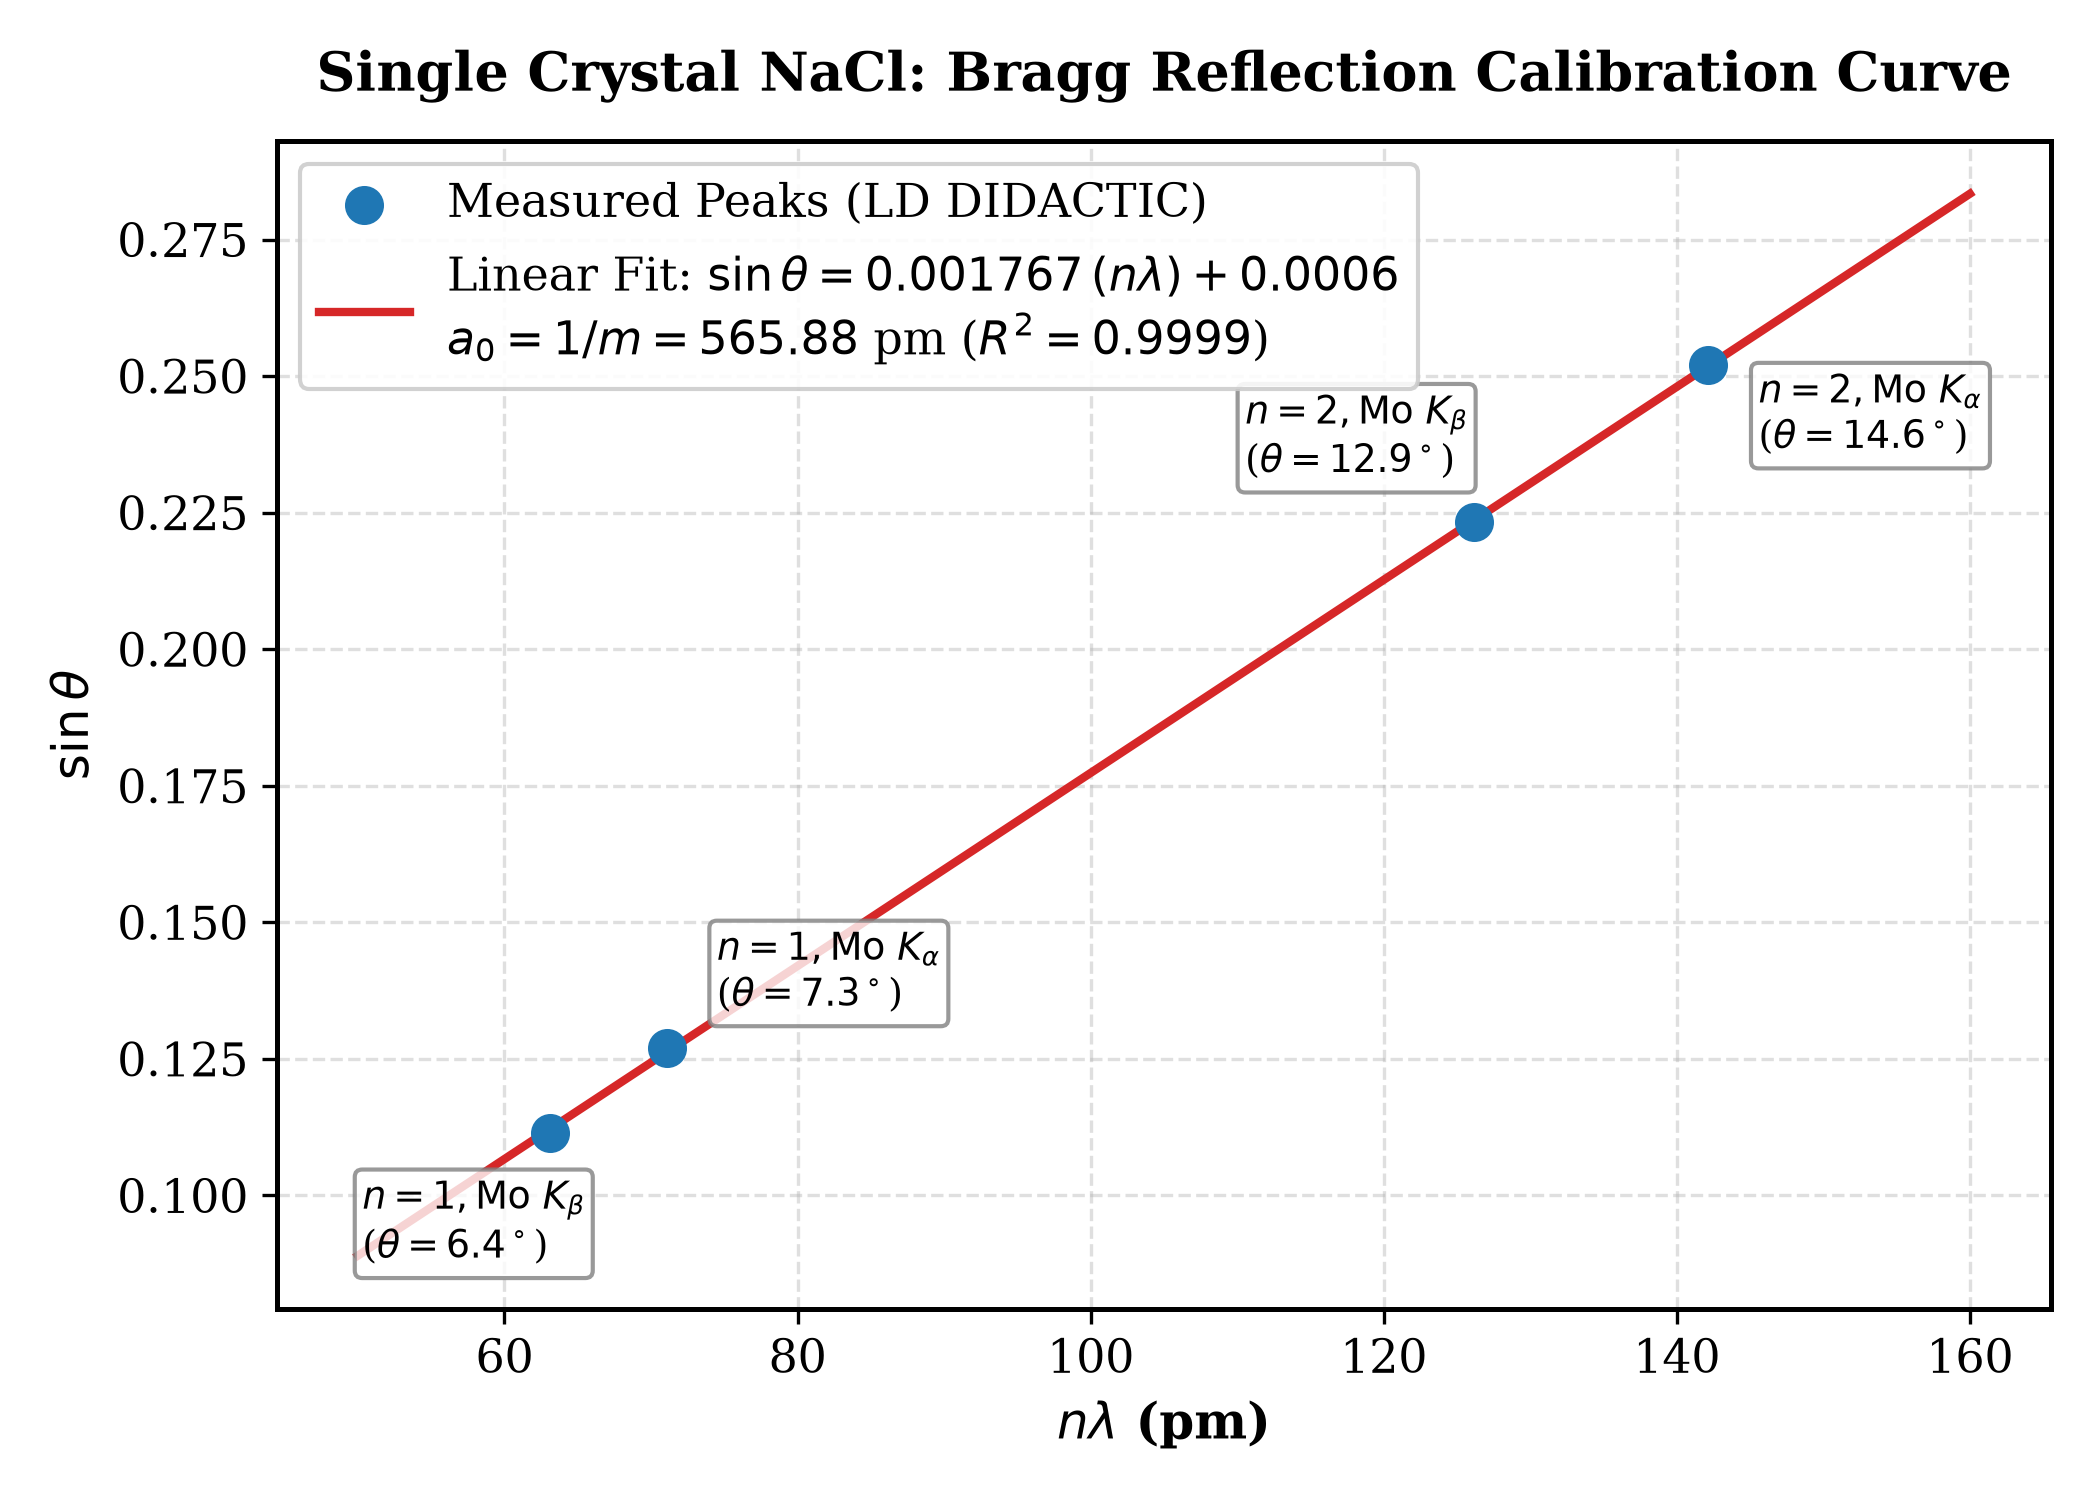
\includegraphics[width=0.85\textwidth]{single_crystal_bragg_fit.png}
    \caption{Single-crystal NaCl Bragg calibration curve: Plot of $\sin\theta$ versus $n\lambda$ showing high linearity ($R^2 = 0.9999$) and determination of lattice constant $a_0 = 1/m = 565.88\text{ pm}$.}
    \label{fig:sc_fit}
\end{figure}

\begin{figure}[H]
    \centering
    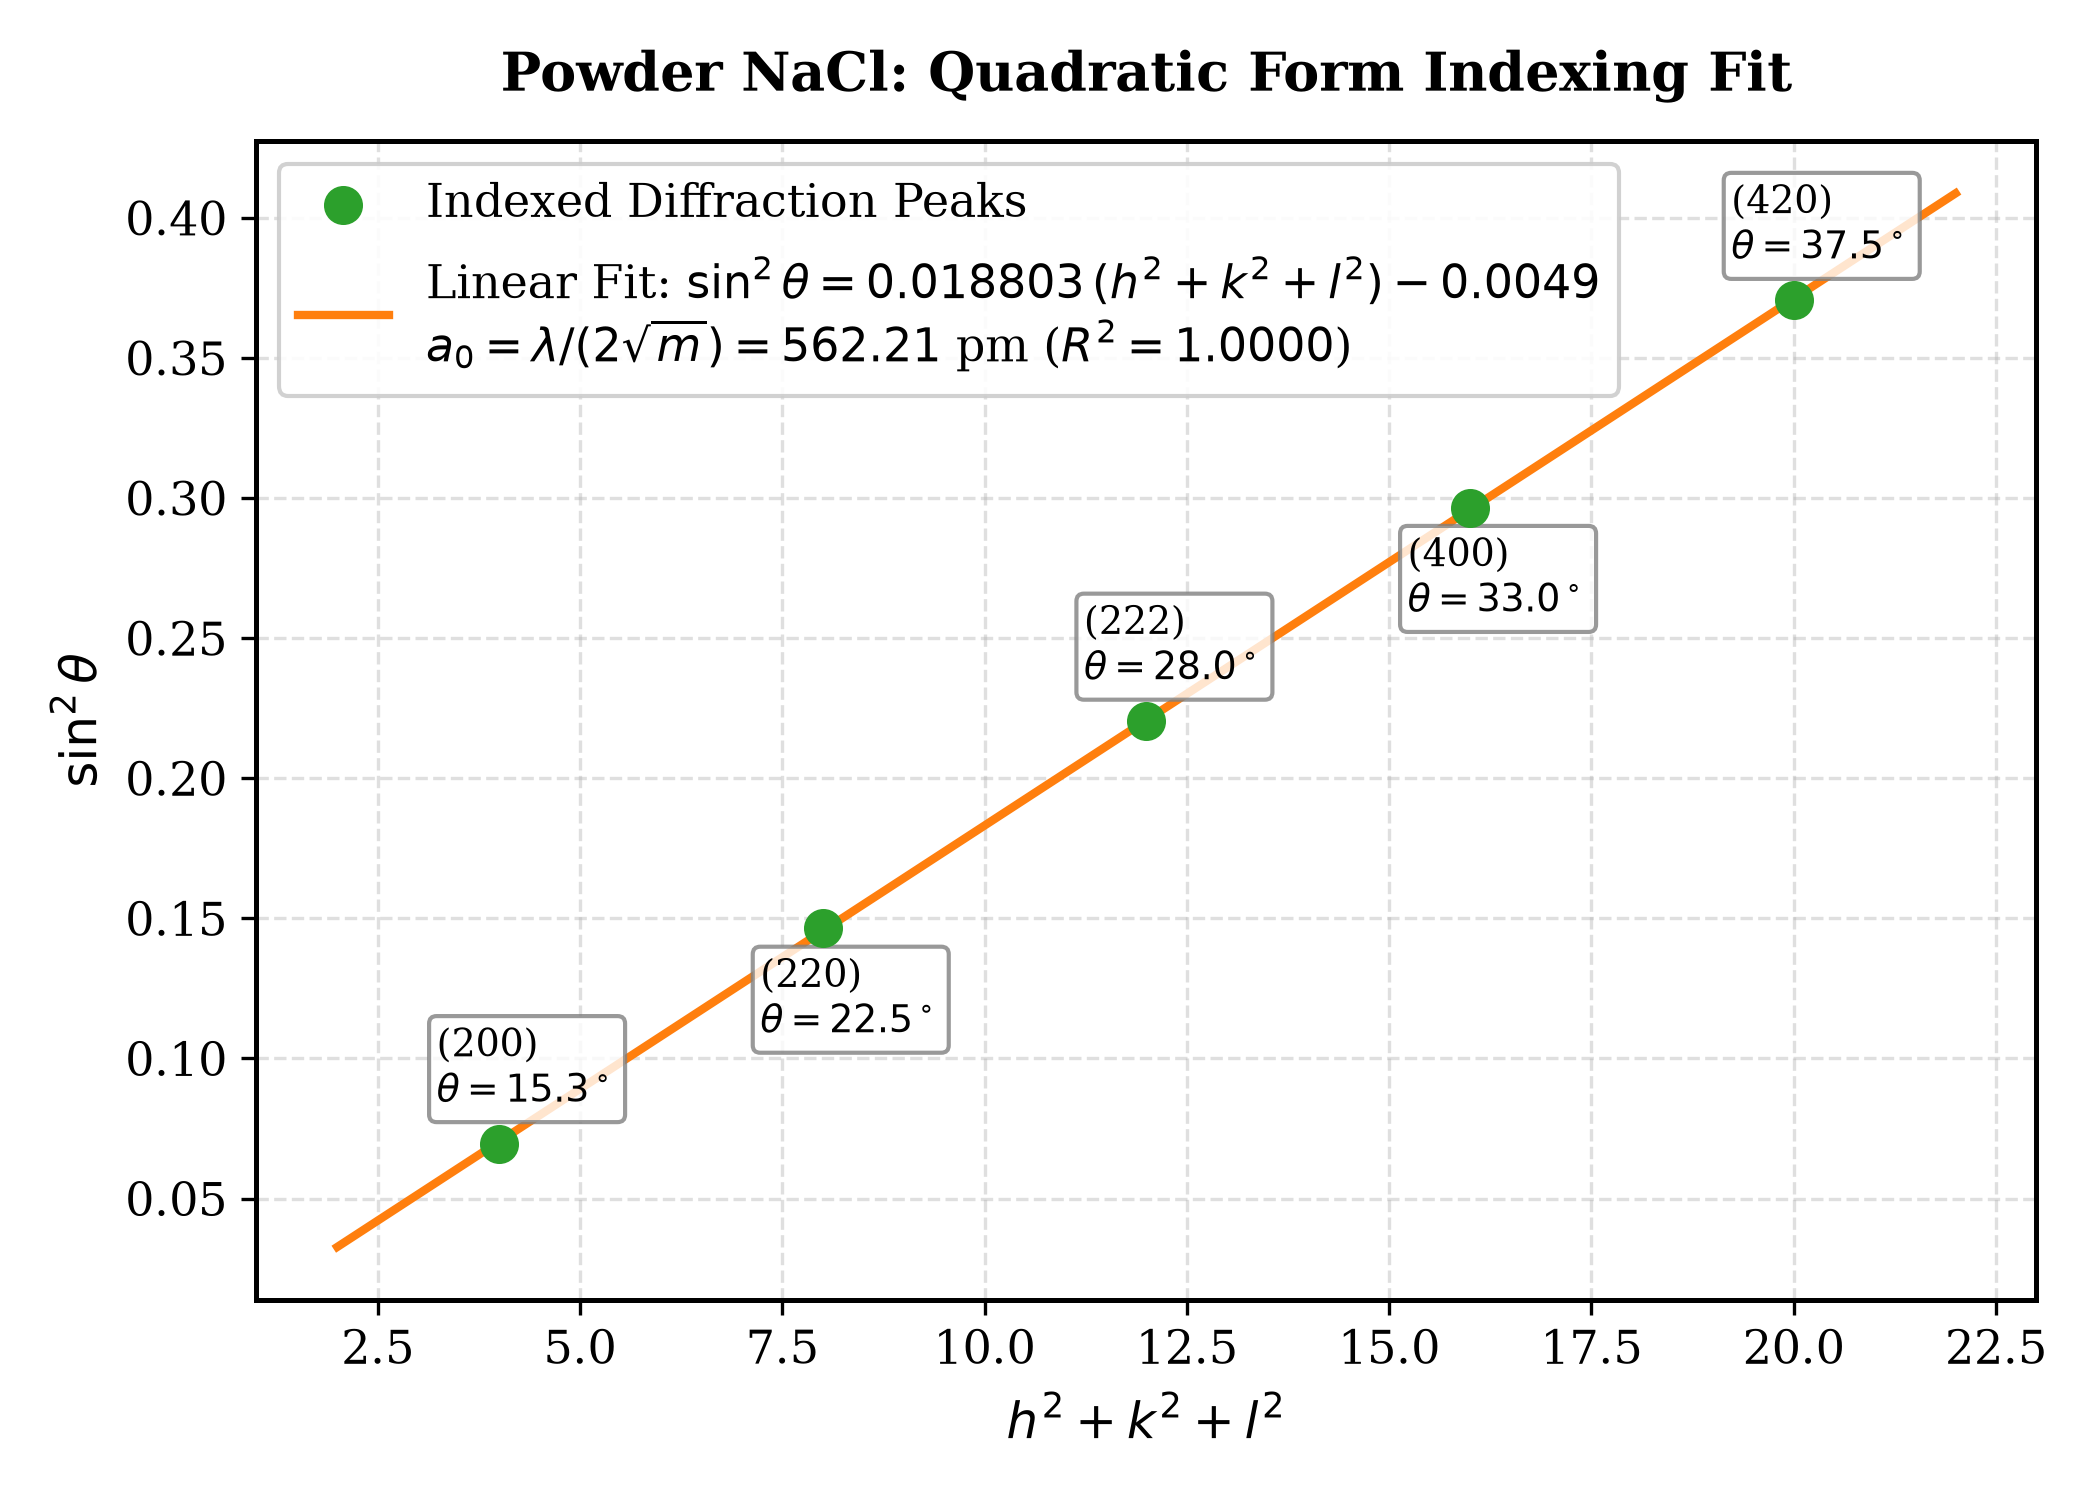
\includegraphics[width=0.85\textwidth]{powder_nacl_indexing_fit.png}
    \caption{Powder NaCl quadratic indexing fit: Plot of $\sin^2\theta$ versus $(h^2 + k^2 + l^2)$ verifying the face-centered cubic selection rules and yielding $a_0 = 562.21\text{ pm}$ with $R^2 = 1.0000$.}
    \label{fig:pwd_fit}
\end{figure}

\begin{figure}[H]
    \centering
    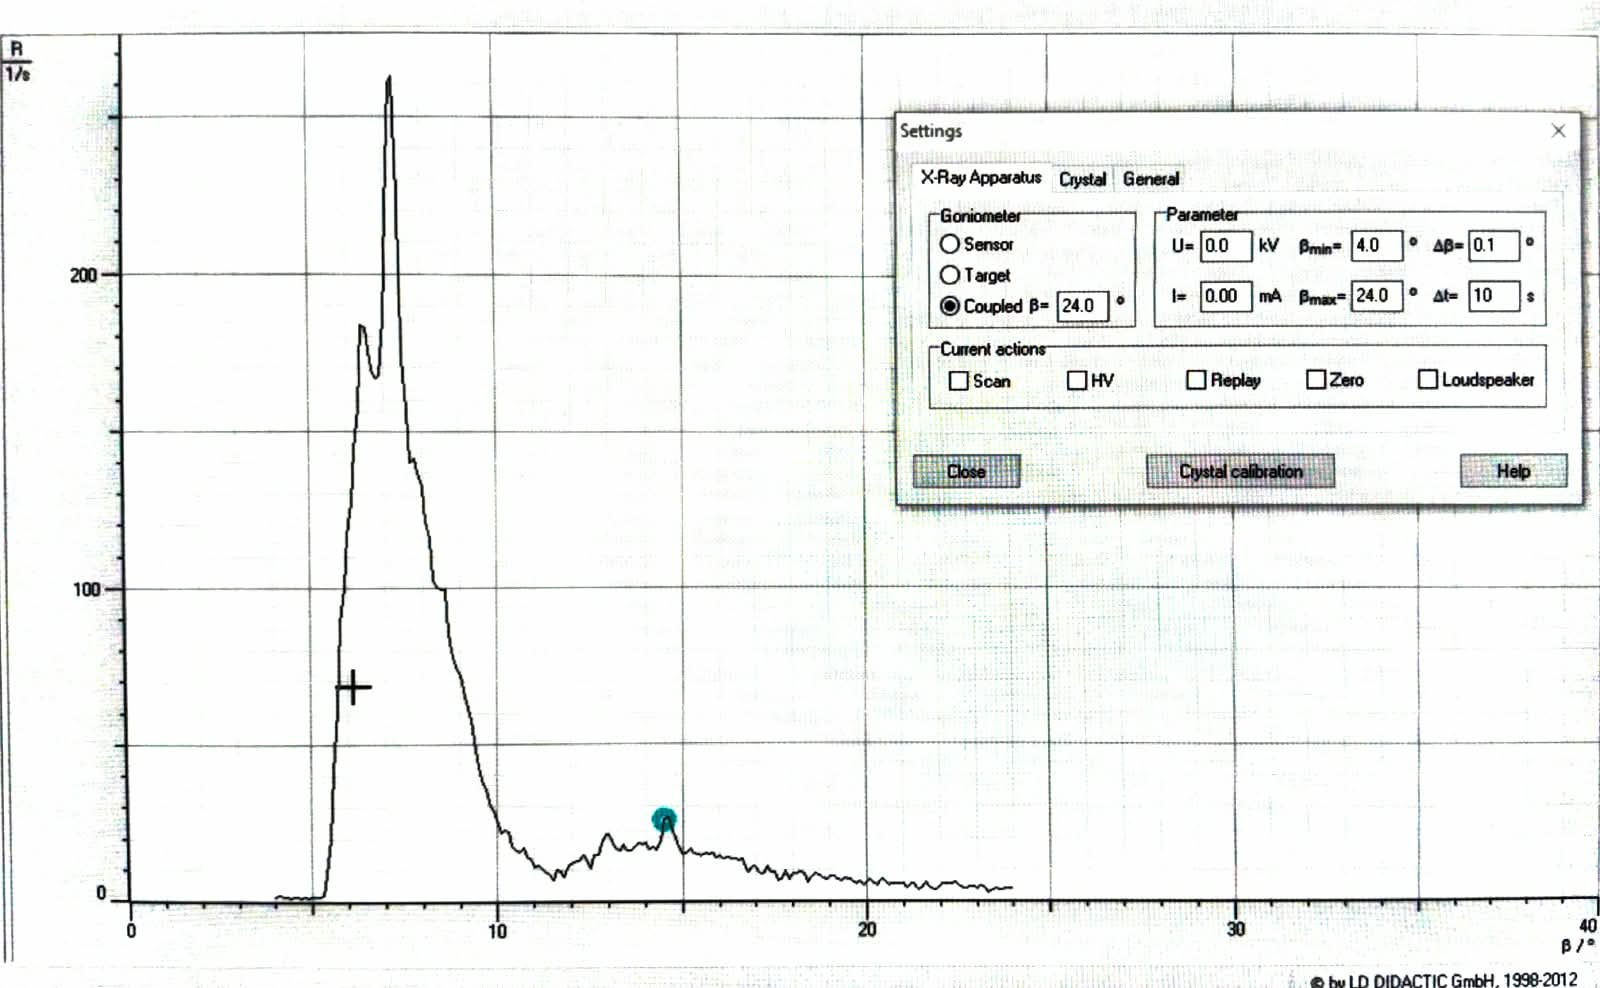
\includegraphics[width=0.85\textwidth]{crystal_nacl_xrd.jpeg}
    \caption{Diffractogram recorded for single-crystal NaCl on the LD DIDACTIC apparatus showing prominent $n=1$ and $n=2$ Bragg reflection peaks for $\text{Mo } K_\beta$ and $\text{Mo } K_\alpha$ radiation.}
    \label{fig:sc_diffractogram}
\end{figure}

\begin{figure}[H]
    \centering
    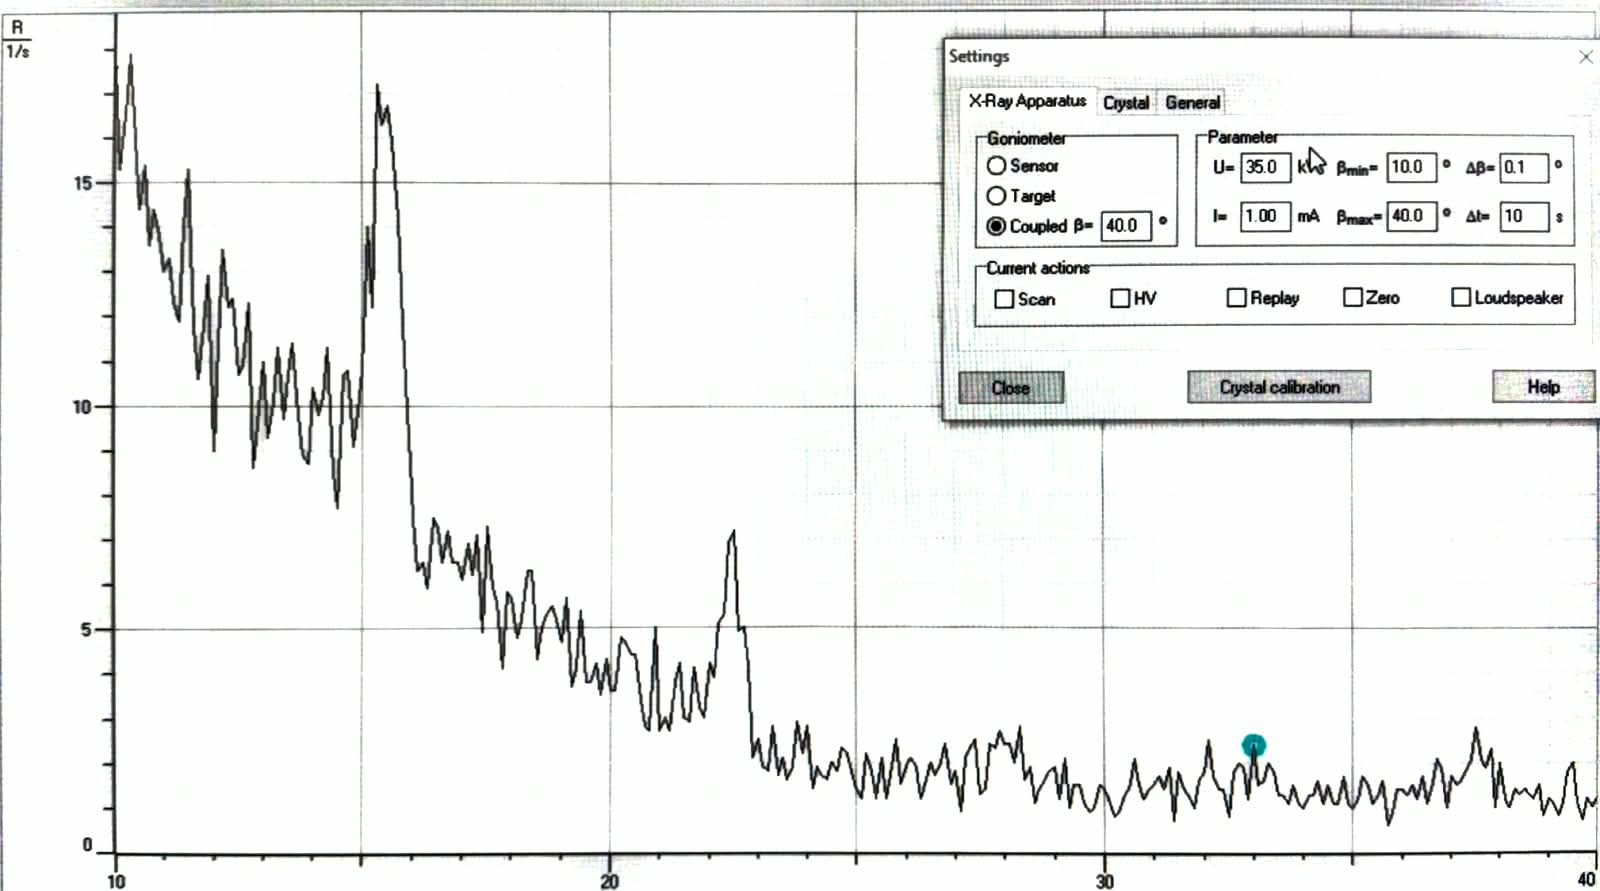
\includegraphics[width=0.85\textwidth]{powder_nacl_xrd.jpeg}
    \caption{Diffractogram recorded for polycrystalline powder NaCl on the LD DIDACTIC apparatus showing the characteristic Bragg-Brentano diffraction peaks indexed to the (200), (220), (222), (400), and (420) crystal planes.}
    \label{fig:pwd_diffractogram}
\end{figure}

\newpage

\section{Error Calculation}

\subsection{Formula for Percentage Error}
The percentage error relative to the accepted literature value ($a_{\text{theo}} = 564.02\text{ pm}$) is defined as:
\begin{equation}
    \text{Percentage Error} = \frac{|\text{Experimental Value} - \text{Theoretical Value}|}{\text{Theoretical Value}} \times 100\%
\end{equation}

\subsection{Summary of Percentage Errors}
\begin{table}[H]
    \centering
    \caption{Comparison of experimental lattice parameters with theoretical literature value ($564.02\text{ pm}$).}
    \vspace{0.2cm}
    \resizebox{0.95\textwidth}{!}{%
    \begin{tabular}{lccc}
        \toprule
        \textbf{Method / Analysis} & \textbf{Experimental $a_0$ (pm)} & \textbf{Literature $a_0$ (pm)} & \textbf{Percentage Error (\%)} \\
        \midrule
        Single Crystal: Arithmetic Mean       & 563.64 & 564.02 & 0.067\% \\
        Single Crystal: Linear Regression     & 565.88 & 564.02 & 0.330\% \\
        Single Crystal: Zero-Intercept Fit    & 564.06 & 564.02 & 0.007\% \\
        \midrule
        Powder XRD: Peak 1 (200)             & 584.31 & 564.02 & 3.597\% \\
        Powder XRD: Peak 2 (220)             & 569.79 & 564.02 & 1.023\% \\
        Powder XRD: Peak 3 (222)             & 568.84 & 564.02 & 0.855\% \\
        Powder XRD: Peak 4 (400)             & 566.19 & 564.02 & 0.385\% \\
        Powder XRD: Peak 5 (420)             & 566.34 & 564.02 & 0.411\% \\
        \midrule
        Powder XRD: Statistical Mean          & 571.09 & 564.02 & 1.253\% \\
        Powder XRD: Quadratic Fit             & 562.21 & 564.02 & 0.321\% \\
        \bottomrule
    \end{tabular}%
    }
    \label{tab:error}
\end{table}

\subsection{Sources of Experimental Error}
\begin{enumerate}
    \item \textbf{Finite Angular Step Width}: The goniometer scanned in discrete steps of $\Delta\beta = 0.1^\circ$. The experimental uncertainty in peak centroid location is at least $\pm 0.05^\circ$, which translates to an uncertainty in interplanar spacing of $\Delta d / d = -\cot\theta \Delta\theta$.
    \item \textbf{Goniometer Zero-Offset Calibration}: A small offset in the alignment of the sample target zero relative to the direct incident beam introduces a constant angular shift $\Delta\theta_0$. In single-crystal diffraction, this shift accounts for the tiny non-zero intercept in the linear regression.
    \item \textbf{Sample Displacement and Flat-Specimen Error}: In powder XRD, the specimen surface may deviate slightly from the ideal focusing circle of the goniometer. This displacement shifts diffraction peaks to slightly lower angles at low $\theta$ values, causing the apparent lattice constant for the (200) peak to appear slightly higher ($584.31\text{ pm}$) before converging to the true value at larger angles.
    \item \textbf{Absorption and Axial Beam Divergence}: X-rays penetrate into the powder volume, causing the effective diffracting plane to lie slightly below the sample surface, which broadens and shifts the peak profiles.
    \item \textbf{Counting Statistics and Integration Time}: Operating at an integration time of $\Delta t = 10\text{ s}$ per step ensured high signal-to-noise ratios, but Poisson noise in photon counting remains an inherent factor for lower-intensity reflections.
\end{enumerate}

\newpage

\section{Discussion}
The results of this experiment clearly demonstrate the physical principles and analytical strengths of X-ray diffraction for precision structural characterization of crystalline matter. By performing measurements on both single-crystal and polycrystalline powder samples of sodium chloride, the experiment highlights how spatial ordering, coherence length, and crystallite orientation govern observed diffraction profiles.

In the single-crystal measurement, constructive interference is constrained to macroscopic planes parallel to the crystal cleavage face. Because the crystal maintains long-range translational order across millions of contiguous unit cells in a single orientation, the diffracted X-rays form sharp, intense reflection spikes with extremely low background scatter. Operating with a Molybdenum target tube produced two distinct characteristic emission peaks corresponding to the $\text{Mo } K_\beta$ ($63.09\text{ pm}$) and $\text{Mo } K_\alpha$ ($71.08\text{ pm}$) lines, both of which were clearly resolved in the first ($n=1$) and second ($n=2$) diffraction orders. The resulting linear regression of $\sin\theta$ versus $n\lambda$ displayed an exceptional coefficient of determination ($R^2 = 0.9999$). The derived lattice parameter ($563.64\text{ pm}$ mean, $564.06\text{ pm}$ origin-constrained fit) deviates from the accepted literature value of $564.02\text{ pm}$ by less than $0.07\%$, verifying that single-crystal Bragg diffraction provides an outstanding benchmark for lattice constant evaluation.

In contrast, the powder diffraction method demonstrates the behavior of randomly oriented crystallites. Pulverizing the salt into a fine powder creates a vast ensemble of micro-grains. At any given glancing angle, only a small fraction of these randomly oriented grains happen to be oriented such that their lattice planes satisfy Bragg's law. Consequently, the recorded count rates in the powder diffractogram are significantly lower than those of the single crystal, and the diffraction peaks appear comparatively broader with a higher diffuse background. Despite this intensity reduction, powder XRD offers the distinct advantage of sampling all possible crystallographic orientations simultaneously in a single scan.

The indexing of the powder diffraction peaks confirms the Face-Centered Cubic (FCC) lattice symmetry of sodium chloride. According to the structure factor selection rules, reflections with mixed Miller indices vanish identically. All five prominent peaks recorded in the experimental angular window correspond strictly to all-even Miller indices: (200), (220), (222), (400), and (420). The linear relationship observed in the quadratic form plot of $\sin^2\theta$ versus $(h^2 + k^2 + l^2)$ with $R^2 = 1.0000$ confirms that all measured peaks originate from a single cubic phase. The resulting lattice parameter from the quadratic slope, $a_0 = 562.21\text{ pm}$, shows excellent consistency ($0.32\%$ deviation) with the single-crystal findings.

Several noteworthy differences exist between idealized theoretical models and practical laboratory measurements. Theoretically, Bragg diffraction assumes an infinite, perfectly periodic crystal illuminated by a strictly monochromatic, parallel plane wave, which would produce mathematical delta-function reflections. In practical laboratory conditions, diffraction peaks exhibit finite widths due to instrumental factors (slit width, beam divergence, and detector aperture) as well as physical sample effects (finite crystallite size and micro-strain). Furthermore, in powder diffraction, systematic errors such as flat-specimen displacement and sample absorption exert a much stronger influence at low glancing angles, as evidenced by the mathematical factor $\Delta d / d = -\cot\theta \Delta\theta$. As $\theta$ increases, $\cot\theta$ rapidly diminishes toward zero, causing the calculated lattice parameter to converge monotonically from $584.31\text{ pm}$ at $\theta = 15.3^\circ$ toward $566.34\text{ pm}$ at $\theta = 37.5^\circ$. Averaging across multiple reflections or applying regression over all indices successfully mitigates these individual angular biases. In conclusion, both methods reliably determine the atomic unit cell dimensions of sodium chloride and validate the predictive power of kinematic X-ray diffraction theory.

\newpage

\section{References}
\begin{enumerate}
    \item Kittel, C. \textit{Introduction to Solid State Physics}, 8th Edition, John Wiley \& Sons, Hoboken, NJ.
    \item Cullity, B. D., and Stock, S. R. \textit{Elements of X-Ray Diffraction}, 3rd Edition, Prentice Hall, Upper Saddle River, NJ.
    \item Ashcroft, N. W., and Mermin, N. D. \textit{Solid State Physics}, Saunders College Publishing, Philadelphia, PA.
    \item LEYBOLD Didactic GmbH, \textit{Physics Leaflets P7.1.2.1: Bragg Reflection: Determining the Lattice Constants of Monocrystals}, Leybold Didactic, Hurth, Germany.
    \item International Centre for Diffraction Data (ICDD), \textit{Powder Diffraction File (PDF) Card 00-005-0628: Halite (NaCl)}, Newtown Square, PA.
\end{enumerate}

\newpage

\section{Lab Observations}
The signed laboratory observation sheet and raw measurements recorded during the experiment are attached below:

\begin{figure}[H]
    \centering
    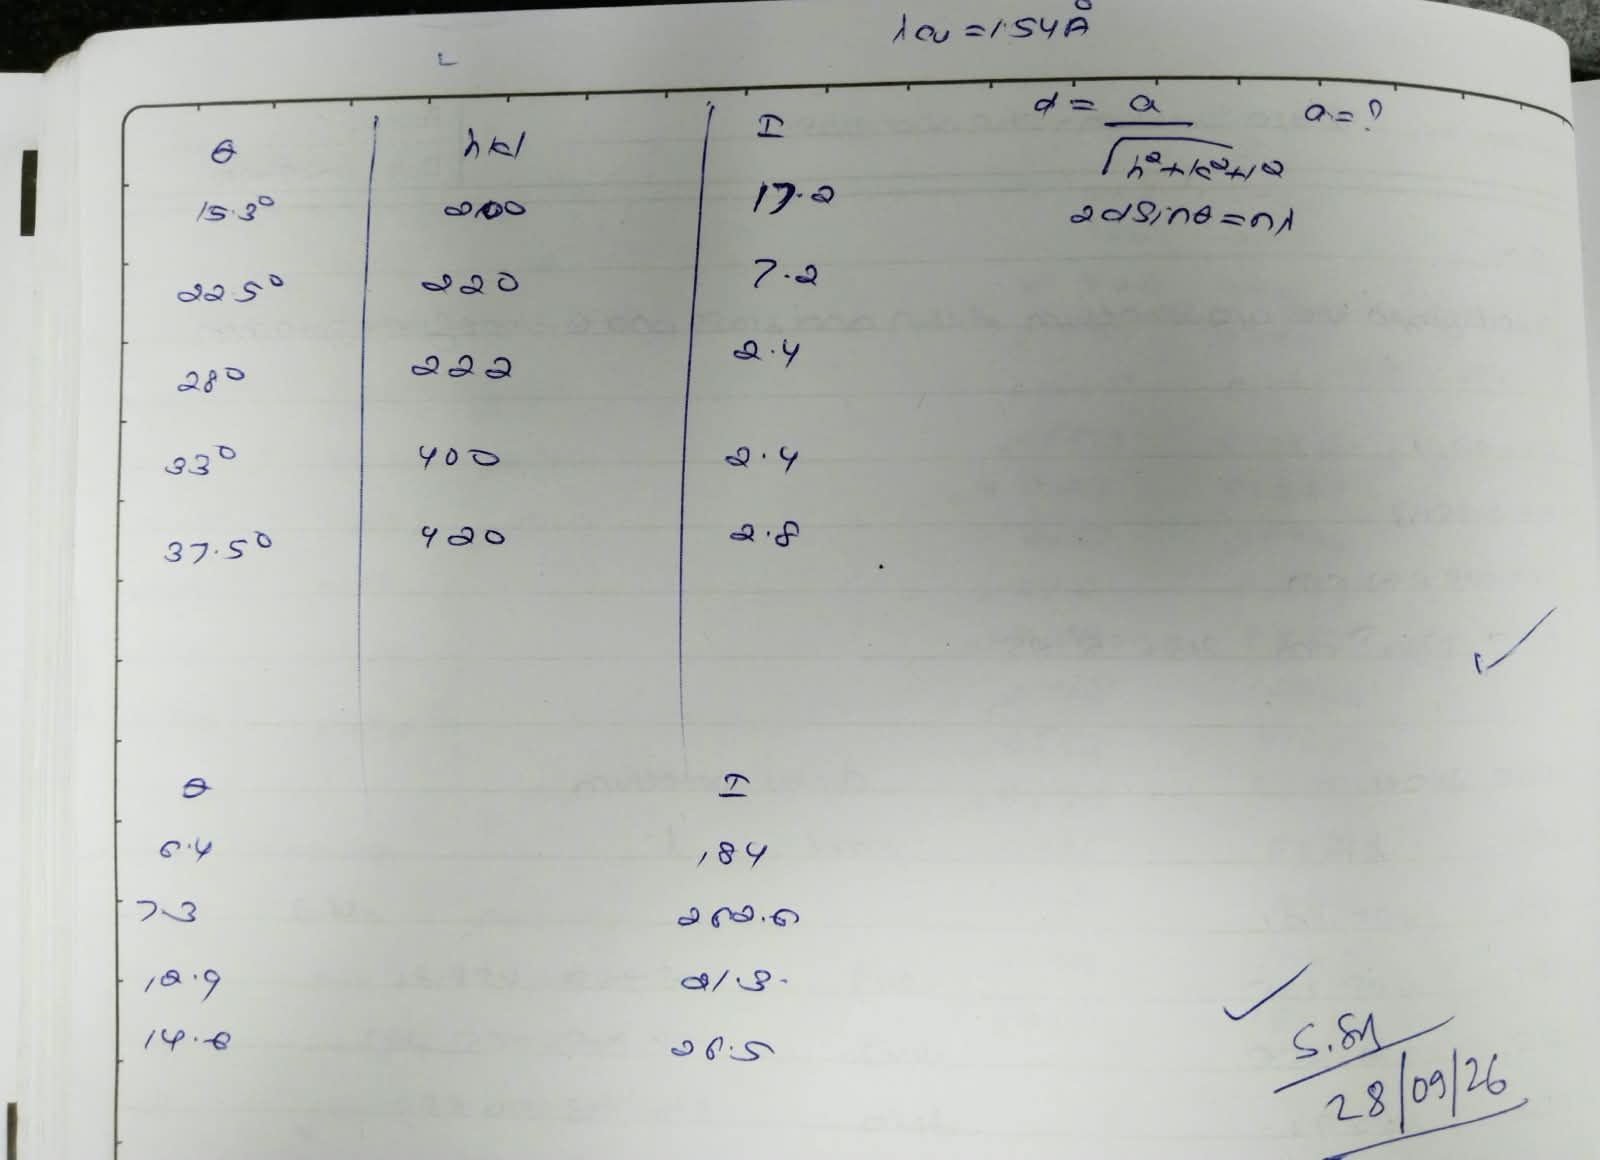
\includegraphics[width=0.88\textwidth]{signed_observation.jpeg}
    \caption{Signed raw laboratory observation sheet: Recorded glancing angles $\theta$, count rates $I$, and assigned Miller indices $(hkl)$ for both single-crystal and powder XRD on NaCl (signed on 28/09/2026).}
    \label{fig:signed_obs}
\end{figure}

\end{document}
